パラメタ同士に相関がある場合, 係数は安定に定まらない. このとき, 回帰係数のノルムに応じた罰則項を加える. これをリッジ回帰といい以下の式で表される.
\begin{align*}
    {\rm min}\left\{ (D\mbox{\boldmath $w$}-\mbox{\boldmath $y$})^{T}(D\mbox{\boldmath $w$}-\mbox{\boldmath $w$})+\lambda \sum_{i=1}^{p}w_{i}^{2}\right\} \tag{2.2}
\end{align*}
パラメタ変数に相関がある、例えば、パラメータ$\mbox{\boldmath $w$}=\left[a \, b\right]^{T}$に関して$a=b$という相関があった場合、
$\mbox{\boldmath $w$}=\left[a\,a\right]^{T}$のように表される。
この時先の例題と同じものを用いて、教師データを$(-2,0),\ (-1,-1),\ (0,1),\ (1,3),\ (2,2)$とするとき, 最小二乗法を用いて線形回帰モデルを求める。
相関がない場合は先の回答のグラフから、$\mbox{\boldmath $W$}=\left[0.8\, 1\right]^{T}$であったが、この解は$a=b$という関係を満たさない。
よって、この相関関係が成り立つと仮定すると、最小の誤差を求めることができず、最小に近い近似の誤差を求めることになるため、下図のように複数の回答が存在する。
\begin{center}
    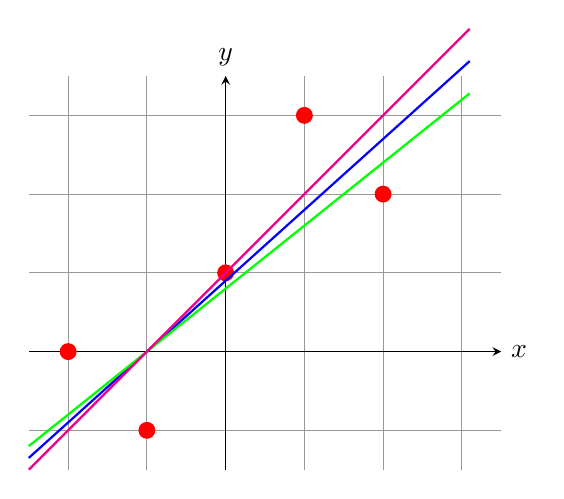
\begin{tikzpicture}[>=stealth]
        \draw[draw=gray!80] (-2.5,-1.5) grid (3.5,3.5);
        \draw[->](-2.5,0)--(3.5,0) node[right] {$x$};
        \draw[->](0,-1.5)--(0,3.5) node[above] {$y$};
        \filldraw[fill=red,draw=red] (-2,0) circle[radius=0.1];
        \filldraw[fill=red,draw=red] (-1,-1) circle[radius=0.1];
        \filldraw[fill=red,draw=red] (0,1) circle[radius=0.1];
        \filldraw[fill=red,draw=red] (1,3) circle[radius=0.1];
        \filldraw[fill=red,draw=red] (2,2) circle[radius=0.1];
        \draw[domain=-2.5:3.1,thick,draw=blue] plot(\x,{\x*0.9+0.9});
        \draw[domain=-2.5:3.1,thick,draw=green] plot(\x,{\x*0.8+0.8});
        \draw[domain=-2.5:3.1,thick,draw=magenta] plot(\x,{\x*1.0+1.0});
    \end{tikzpicture}
\end{center}
そのため、元の誤差の式だけでは、収束値が一定しない可能性があるが、一つの考え方として、パラメータベクトルの長さが一番最小となるとき、最小の誤差であると考えると、罰則項として、ノルムを加えることで収束先が一定し、最小誤差が特定できるようにする
というものである。\\
このようにして、収束しない可能性のある目的関数を収束するような関数に変換することを{\bf 正則化}という